\chapter{Sketch Simplification}

Sketch Simplification refers to automatically converts rough sketches into simplified clean drawings. It is one of the most fundamental task because it is the first step into the whole of the pipeline. An accurate and fast method is required to provide solid foundation for subsequent processing. However, as we will see, it is a relatively under-explored area and we yet to see a fast and high quality procedure for this tasks. As such, it is expected to be the most research intensive area for future development. Nevertheless, the task itself is relative straight forward and similar problems have developed mature solutions, therefore it is not expected to be difficult. I will also propose a number of possible directions for future experiments.

\label{chapterlabel4}
\section{Approaches \& Methods}
Traditionally, rough sketches are iteratively refined by the artist himself/herself. This requires manually tracing the rough sketch repeatedly to produce a clean and satisfying drawing. This process is tedious, time-consuming and involve a large overhead. There have been some methods proposed to simplify sketch drawings. Some assists user to clean up sketches based on geometry relationships between strokes\cite{fiserShipShapeDrawingBeautification2015} and fitting stroke using Bezier Curves\cite{baeILoveSketchAsnaturalaspossibleSketching2008}; Others simplify rough lines by removing unnecessary ones\cite{liuClosureawareSketchSimplification2015}. However, these traditional methods neither change the way artists clean up sketches, nor provide a fully automatic way to simplify them. Moreover, they often operate on vector graphics, which is more dominate in the design industry and not the 2D animation industry.

As far as I know, the first attempt to simplify sketches in a fully automatic way on raster images was in 2016\cite{simo-serraLearningSimplifyFully2016}. The researchers used an encoder-decoder CNN architecture and achieved reasonable result. Worth-mentioning, they used a loss map which assign higher weighting to lines and achieved much faster training. Their results showed that for simple sketches the model is able to produce accurate strokes (see figure \ref{fig:learning2simp}).

\begin{figure}
    \centering
    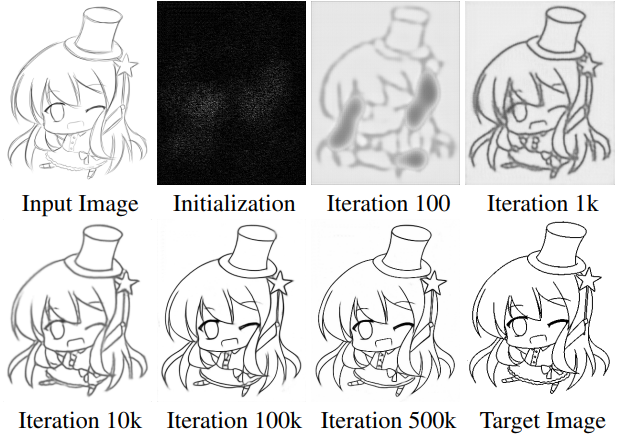
\includegraphics[width=0.75\textwidth]{images/sketch/learning2simp.png}
    \caption{Visualization of the output image as training proceeds for encoder-decoder CNN model.} 
    \label{fig:learning2simp}
\end{figure}


\section{Design \& Implementation}
